\documentclass[12pt]{article}
\usepackage{fontspec} % 字型
\setmainfont{Taipei Sans TC Beta}
\usepackage{xeCJK} % 字型
\setCJKmainfont{Taipei Sans TC Beta}
\usepackage[top=1cm, bottom=1cm, left=1cm, right=1cm]{geometry} % 頁面設定
% \usepackage{indentfirst} % 首行縮排
\renewcommand{\baselinestretch}{1.5}
\pagenumbering{gobble} % 無頁碼
\usepackage{enumitem} % 列表縮排
\usepackage{zhnumber} % 中文數字
\usepackage{graphicx}
\usepackage{float}

\begin{document}

\section*{pA:STring}

\begin{itemize}[label={}, itemsep=0pt]
    \item 給你一個字串 $s$,重複執行以下的操作:刪除最左邊為\ "\textbf{ST}"\ 子字串,如果沒有就停止,並輸出剩餘字串的長度
    \item 測資範圍:$2 \leq \mid s \mid \leq 2 \times 10^5$,$\mid s \mid$ 為偶數,S 和 T 的數量相同
    \item 範例測資:
    \item 
    \centering
    \begin{tabular}{|c|c|c|c|}
        \hline
        input  & TSTTSS & SSTTST & TSSTTTSS \\ \hline
        output & 4      & 0      & 4        \\ \hline
    \end{tabular}
\end{itemize}

\section*{pB:括號配對}

\begin{itemize}[label={}, itemsep=0pt]
    \item 給你一個字串 $s$,只由 <\ > (\ ) [\ ] \{\ \} 組成,左括號之間可以互相替換,右括號同理,請判斷 $s$ 是否可以變成合法的括號序列,如果可以就輸出最少的替換次數,否則輸出\ "\textbf{Impossible}"
    \item 測資範圍:$0 \leq \mid s \mid \leq 2 \times 10^6$
    \item 範例測資:
    \item
    \centering
    \begin{tabular}{|c|c|c|c|}
        \hline
        input  & [\ <\ \}\ )\ \{\ \} & \ \{\ (\ )\ \}\ [\ ] & \ ]\ ]     \\ \hline
        output & 2                   & 0                    & Impossible \\ \hline
    \end{tabular}
\end{itemize}

\section*{pC:最近較小數字}

\begin{itemize}[label={}, itemsep=0pt]
    \item 給你一個字串 $n$ 個數字 $a_i$(based-1),請對於每個 $a_i$ 在它左邊且比它小的最近位置
    \item 測資範圍:$1 \leq n \leq 2 \times 10^5$,$1 \leq a_i \leq 10^9$
    \item 範例測資:
    \item 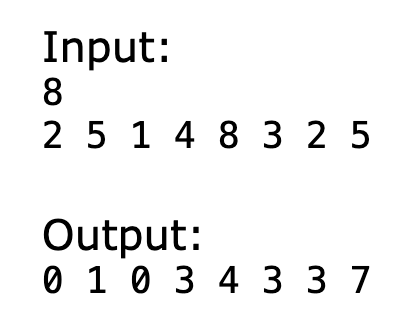
\includegraphics[width=5.0cm]{img/pC}
\end{itemize}

\pagebreak

\section*{pD:儲存站}

\begin{itemize}[label={}, itemsep=0pt]
    \item 有一個無限容量的儲存站,貨物只會左進右出,並且相對順序不會改變,接下來有 $q$ 個操作
    \begin{itemize}[label={-}, itemsep=0pt]
        \item $1\ x\ c$:把 $c$ 個價值為 $x$ 的貨物放進儲存站
        \item $2\ c$:把 $c$ 個貨物取出,並計算貨物的總價價值
    \end{itemize}
    \item 測資範圍:$1 \leq q \leq 2 \times 10^5$,$0 \leq x \leq 10^9$,$1 \leq c \leq 10^9$
    \item 範例測資:
    \item
    \centering
    \begin{tabular}{|l|l|l|l|}
        \hline
        \multicolumn{1}{|c|}{input}  & 4     & 2                       & 5     \\
                                     & 1 2 3 & 1 1000000000 1000000000 & 1 1 1 \\
                                     & 2 2   & 2 100000000             & 1 1 1 \\
                                     & 1 3 4 &                         & 1 1 1 \\
                                     & 2 3   &                         & 1 1 1 \\
                                     &       &                         & 1 1 1 \\ \hline
        \multicolumn{1}{|c|}{output} & 4     & 1000000000000000000     &       \\
                                     & 8     &                         &       \\ \hline
    \end{tabular}
\end{itemize}

\section*{pE:LR 排列}

\begin{itemize}[label={}, itemsep=0pt]
    \item 你有一個字串 $s$,對於一個陣列 $V=\{0\}$,對於每個 $i$ 操作如下
    \begin{itemize}[label={-}, itemsep=0pt]
        \item $s_i = `L'$:把 $i$ 插入在 $i-1$ 的左邊
        \item $s_i = `R'$:把 $i$ 插入在 $i-1$ 的右邊
    \end{itemize}
    \item 測資範圍:$1 \leq q \leq 5 \times 10^5$,$\mid s \mid = n$,$s$ 僅由 `L' 和 `R' 組成
    \item 範例測資:
    \item
    \centering
    \begin{tabular}{|c|l|l|}
        \hline
        input                  & 5           & 7               \\
        \multicolumn{1}{|l|}{} & LRRLR       & LLLLLLL         \\ \hline
        output                 & 1 2 4 5 3 0 & 7 6 5 4 3 2 1 0 \\ \hline
    \end{tabular}
\end{itemize}

\end{document}